\documentclass[10pt,french]{book}

\input philippe2013


\entete{\seconde 7}{Statistiques continues}{A}
\RegleEntete
\pieddepage{}{}{}

\newcommand\presentation{
\setcounter{exo}{0}
    \begin{tabular}{ll}
        Nom : \\[5pt]
        Prénom :
    \end{tabular}
\hfill
    \textbf{Note :}
        \renewcommand\arraystretch{2.3}
    \begin{tabular}{|c|}
        \hline
            \slashbox{\Huge\bfseries\phantom{10}}{\Huge\bfseries 10}\\
        \hline
    \end{tabular}
        \renewcommand\arraystretch{1.5}\par\bigskip
    \hrulefill\par\vspace{1cm}
}


\begin{document}


%-------------
% SUJET A
%-------------

\presentation

Le maire d'une petite ville réalise une étude complète pour savoir quel est le temps de trajet des habitants de la ville entre chez eux et leur travail.\par Voilà les résultats obtenus :

\begin{center}
\renewcommand\arraystretch{2}
    \begin{tabular}{*{8}{|>{\centering\arraybackslash}m{1.5cm}}|}
        \hline
            Temps \par en min & $\intervallefo{0}{10}$ & $\intervallefo{10}{20}$ & $\intervallefo{20}{25}$ & $\intervallefo{25}{30}$ & $\intervallefo{30}{40}$ & $\intervallefo{40}{60}$  & Total \\
        \hline
            Centre\par de classe & & & & & & & xxx\\
        \hline
            Effectif & 5 & 10 & 20 & 30 & 20 & 40 & \\
        \hline
            {\small Fréquence \par en \%} & & & & & & & \\
        \hline
            {\small Fréquence \par Cumulée \par Croissante} & & & & & & & xxx \\
        \hline
    \end{tabular}
\end{center}

\begin{enumerate}
    \item Compléter le tableau sans arrondir les fréquences.
    \item Calculer le temps de trajet moyen en minutes. Arrondir à l'unité si nécessaire.
    \item Construire ci-dessous l'histogramme de cette série statistique. \textbf{Attention à l'unité d'aire}.
\end{enumerate}

\begin{center}
\begin{tikzpicture}[>=latex]
	% Dimensions du repere
	\def\xmin{0} \def\xmax{13} \def\ymin{0} \def\ymax{7}
	% Grilles
    \draw [xstep=1,ystep=0.5,gray,line width = 0.7pt,dashed] (\xmin,\ymin) grid (\xmax,\ymax);
	\draw [xstep=1,ystep=1,gray,line width = 1pt] (\xmin,\ymin) grid (\xmax,\ymax);
    \draw (6.5,-1) node {Histogramme};
    \draw[pattern=north east lines,line width = 1.5pt] (0,6) rectangle (2,7);
    \draw (2,6.5) node[right] {= 10 personnes};
    \draw[line width = 0.7,->] (0,0) -- (13,0) node[below] {\small Temps en minutes};
    \foreach \x in {0,10,...,50} \draw ({\x/5},3pt)--({\x/5},-3pt) node[below] {$\x$};
\end{tikzpicture}
\end{center}

\begin{enumerate}[resume]
    \item Tracer si contre le polygone des fréquences cumulées croissantes.
    \item Graphiquement, en laissant apparaître les pointillés, déterminer la valeur de la médiane $M_e$, du premier et du troisième quartile $Q_1$ et $Q_3$. \textbf{Répondre à la question par une phrase}.
    \item En déterminant l'équation réduite d'une droite, déterminer une valeur plus précise de la médiane par le calcul. Arrondir le résultat final à l'unité. Donner une interprétation.
\end{enumerate}

\clearpage

\begin{center}
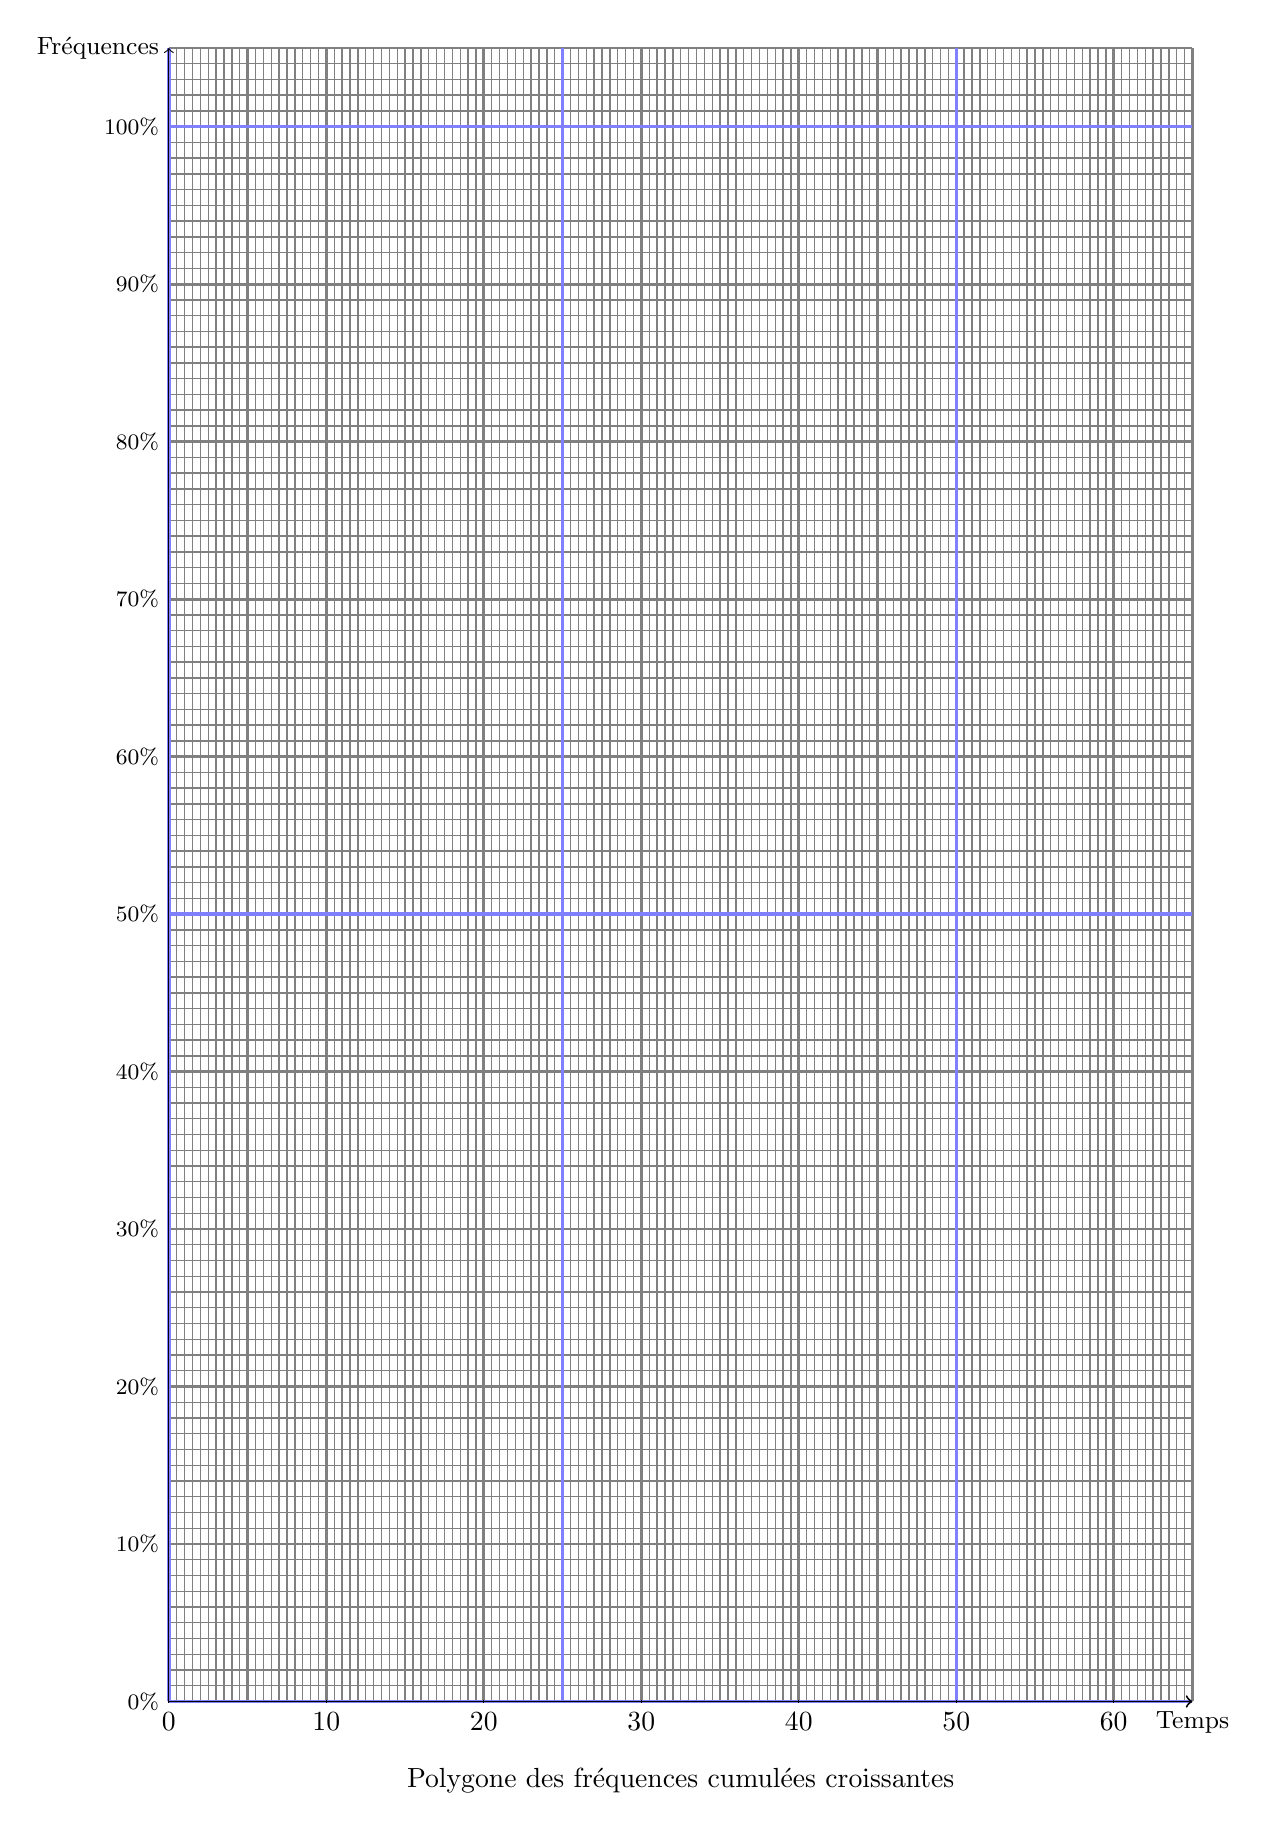
\begin{tikzpicture}[yscale=0.2]
	% Dimensions du repere
	\def\xmin{0} \def\xmax{13} \def\ymin{0} \def\ymax{105}
	% Grilles
	\draw [xstep=0.1,ystep=1,gray,line width = 0.5pt]  (\xmin,\ymin) grid (\xmax,\ymax);
	\draw [xstep=1,ystep=10,gray,line width = 1pt] (\xmin,\ymin) grid (\xmax,\ymax);
	\draw [xstep=5,ystep=50,line width = 1.2pt,color=blue!50]  (\xmin,\ymin) grid (\xmax,\ymax);
    \draw (6.5,-5) node {Polygone des fréquences cumulées croissantes};
    \draw[<-] (0,105) node[left] {\small Fréquences} -- (0,0);
    \draw[line width = 0.7,->] (0,0) -- (13,0) node[below] {\small Temps};
    \foreach \x in {0,10,...,60} \draw ({\x/5},3pt)--({\x/5},-3pt) node[below] {$\x$};
    \foreach \x in {0,10,...,100} \draw (0,\x) node[left] {\footnotesize $\x\%$};
\end{tikzpicture}
\end{center}\clearpage

%-------------
% SUJET B
%-------------
\entete{\seconde 7}{Statistiques continues}{B}

\presentation

Le marie d'une petite ville réalise une étude complète pour savoir quel est le temps de trajet des habitants de la ville entre chez eux et leur travail.\par Voilà les résultats obtenus :

\begin{center}
\renewcommand\arraystretch{2}
    \begin{tabular}{*{8}{|>{\centering\arraybackslash}m{1.5cm}}|}
        \hline
            Temps \par en min & $\intervallefo{0}{10}$ & $\intervallefo{10}{20}$ & $\intervallefo{20}{25}$ & $\intervallefo{25}{30}$ & $\intervallefo{30}{40}$ & $\intervallefo{40}{60}$  & Total \\
        \hline
            Centre\par de classe & & & & & & & xxx\\
        \hline
            Effectif & 5 & 20 & 30 & 10 & 20 & 40 & \\
        \hline
            {\small Fréquence \par en \%} & & & & & & & \\
        \hline
            {\small Fréquence \par Cumulée \par Croissante} & & & & & & & xxx \\
        \hline
    \end{tabular}
\end{center}

\begin{enumerate}
    \item Compléter le tableau sans arrondir les fréquences.
    \item Calculer le temps de trajet moyen en minutes. Arrondir à l'unité si nécessaire.
    \item Construire ci-dessous l'histogramme de cette série statistique. \textbf{Attention à l'unité d'aire}.
\end{enumerate}

\begin{center}
\begin{tikzpicture}[>=latex]
	% Dimensions du repere
	\def\xmin{0} \def\xmax{13} \def\ymin{0} \def\ymax{7}
	% Grilles
    \draw [xstep=1,ystep=0.5,gray,line width = 0.7pt,dashed] (\xmin,\ymin) grid (\xmax,\ymax);
	\draw [xstep=1,ystep=1,gray,line width = 1pt] (\xmin,\ymin) grid (\xmax,\ymax);
    \draw (6.5,-1) node {Histogramme};
    \draw[pattern=north east lines,line width = 1.5pt] (0,6) rectangle (2,7);
    \draw (2,6.5) node[right] {= 10 personnes};
    \draw[line width = 0.7,->] (0,0) -- (13,0) node[below] {\small Temps en minutes};
    \foreach \x in {0,10,...,50} \draw ({\x/5},3pt)--({\x/5},-3pt) node[below] {$\x$};
\end{tikzpicture}
\end{center}

\begin{enumerate}[resume]
    \item Tracer si contre le polygone des fréquences cumulées croissantes.
    \item Graphiquement, en laissant apparaître les pointillés, déterminer la valeur de la médiane $M_e$, du premier et du troisième quartile $Q_1$ et $Q_3$. \textbf{Répondre à la question par une phrase}.
    \item En déterminant l'équation réduite d'une droite, déterminer une valeur plus précise de la médiane par le calcul. Arrondir le résultat final à l'unité. Donner une interprétation.
\end{enumerate}

\clearpage

\begin{center}
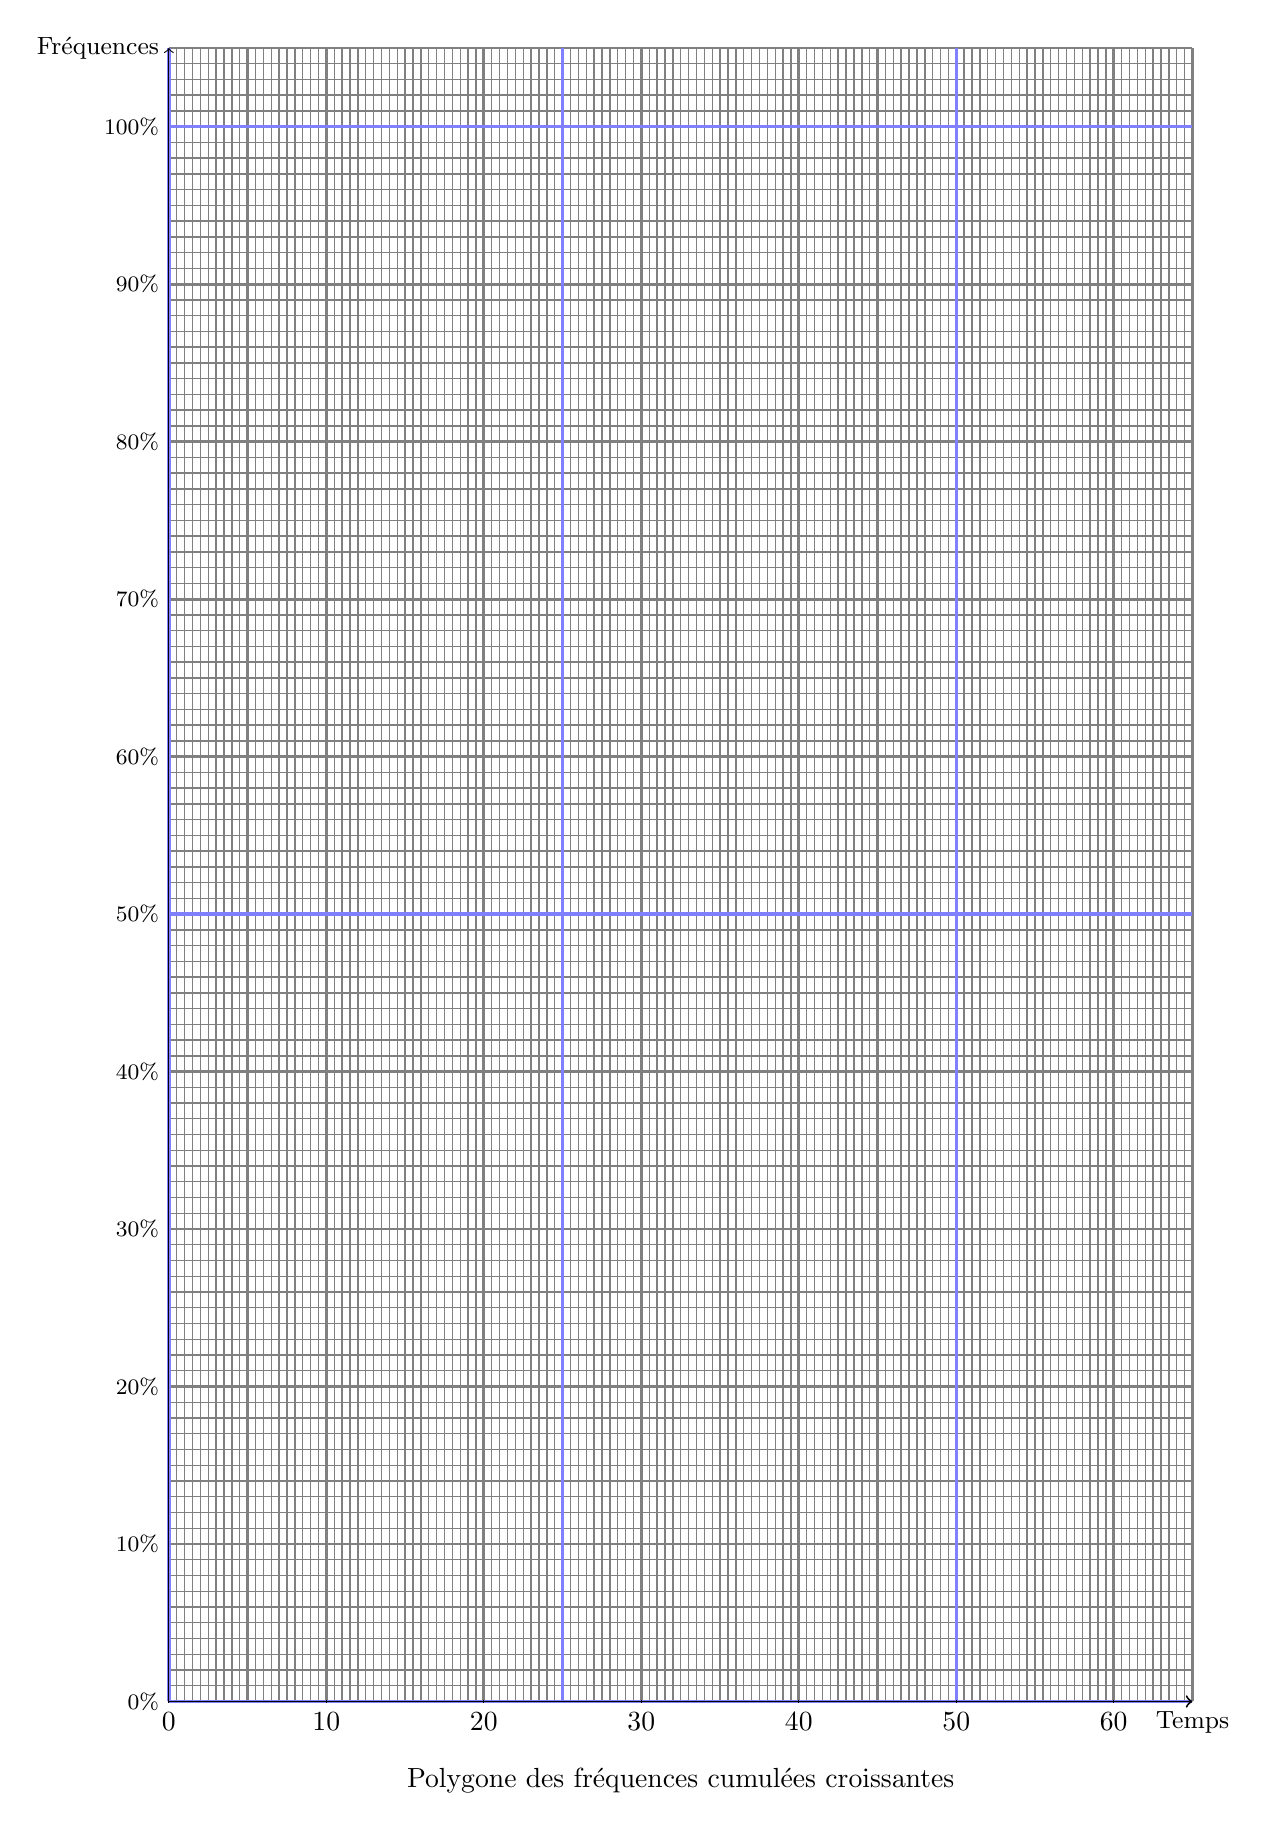
\begin{tikzpicture}[yscale=0.2]
	% Dimensions du repere
	\def\xmin{0} \def\xmax{13} \def\ymin{0} \def\ymax{105}
	% Grilles
	\draw [xstep=0.1,ystep=1,gray,line width = 0.5pt]  (\xmin,\ymin) grid (\xmax,\ymax);
	\draw [xstep=1,ystep=10,gray,line width = 1pt] (\xmin,\ymin) grid (\xmax,\ymax);
	\draw [xstep=5,ystep=50,line width = 1.2pt,color=blue!50]  (\xmin,\ymin) grid (\xmax,\ymax);
    \draw (6.5,-5) node {Polygone des fréquences cumulées croissantes};
    \draw[<-] (0,105) node[left] {\small Fréquences} -- (0,0);
    \draw[line width = 0.7,->] (0,0) -- (13,0) node[below] {\small Temps};
    \foreach \x in {0,10,...,60} \draw ({\x/5},3pt)--({\x/5},-3pt) node[below] {$\x$};
    \foreach \x in {0,10,...,100} \draw (0,\x) node[left] {\footnotesize $\x\%$};
\end{tikzpicture}
\end{center}\clearpage


\end{document}
